\section{Results}

\subsection{Model Performance}

Table~\ref{tab:performance_metrics} summarizes the performance of our two base classifiers (CNN8 and VGG-inspired) alongside their final ensemble. Although the individual models reached 77.8\% and 79.2\% accuracy on the validation split, the ensemble delivered superior real-world results---achieving 78.6\% on the Kaggle public test and 76.7\% on the private holdout---outperforming the best single model by over two percentage points and demonstrating the clear benefit of combining their complementary strengths.

\begin{table}[h!]
\centering
\caption{Comparative performance of the baseline CNN8, VGG-inspired model, and their final ensemble.}
\label{tab:performance_metrics}
\resizebox{\columnwidth}{!}{
  \begin{tabular}{@{}lccccc|cc@{}}
    \toprule
      \multirow{2}{*}{\textbf{Model}}
      & \multicolumn{5}{c|}{\textbf{Validation}} 
      & \multicolumn{2}{c}{\textbf{Test (Acc.)}} \\
    \cmidrule(lr){2-6}\cmidrule(l){7-8}
      & Acc. & AUC & Prec. & Rec. & F1 
      & Public & Private \\
    \midrule
    CNN8 & 0.778 & 0.831 & 0.780 & 0.775 & 0.777  & 0.761 & 0.737  \\
    VGG-inspired   & 0.792 & 0.845 & 0.796 & 0.789 & 0.792 & 0.771 & 0.747 \\
    \midrule
    Ensemble &   --   &  --   &   --   &   --   &   --   & \textbf{0.786} & \textbf{0.767} \\
    \bottomrule
  \end{tabular}
}
\end{table}

Also, data augmentation with CutMix and MixUp boosted our test‐set accuracy from 72.0\% (public) and 69.3\% (private) to 78.6\% and 76.7\%, respectively---an improvement of over two percentage points versus the best individual model (Fig.~\ref{fig:augmentation_result}).

\begin{figure}[h!]
  \centering
  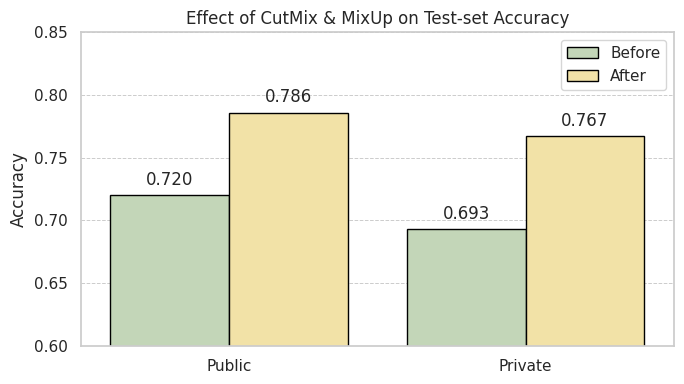
\includegraphics[width=\columnwidth]{figures/augmentation_result}
  \caption{Impact of CutMix and MixUp augmentation on Kaggle test‐set accuracy. “Before” refers to the baseline (72.0\% public / 69.3\% private); “After” shows the augmented results (78.6\% public / 76.7 \% private).}
  \label{fig:augmentation_result}
\end{figure}